\documentclass[aspectratio=169,10pt]{beamer}

\usepackage[T1]{fontenc}
\usepackage{lmodern}
\usepackage{amsmath}
\usepackage{booktabs}
\usepackage{array}
\usepackage{tikz}
\usetikzlibrary{arrows.meta,calc,positioning,patterns,shapes.geometric}

\definecolor{Navy}{HTML}{17324D}
\definecolor{Blue}{HTML}{2474B5}
\definecolor{Teal}{HTML}{18A999}
\definecolor{Green}{HTML}{4C956C}
\definecolor{Yellow}{HTML}{F3C969}
\definecolor{Orange}{HTML}{E07A5F}
\definecolor{Purple}{HTML}{76549A}
\definecolor{Light}{HTML}{F4F7FA}
\definecolor{Mid}{HTML}{D8E2EA}
\definecolor{DarkGrey}{HTML}{536471}
\definecolor{Danger}{HTML}{B33A3A}

\setbeamercolor{normal text}{fg=Navy,bg=white}
\setbeamercolor{frametitle}{fg=white,bg=Navy}
\setbeamercolor{title}{fg=Navy}
\setbeamercolor{structure}{fg=Blue}
\setbeamercolor{block title}{fg=white,bg=Blue}
\setbeamercolor{block body}{fg=Navy,bg=Light}
\setbeamertemplate{navigation symbols}{}
\setbeamertemplate{itemize item}{\color{Teal}$\blacktriangleright$}
\setbeamertemplate{itemize subitem}{\color{Blue}$\bullet$}
\setbeamertemplate{frametitle}{%
  \nointerlineskip\begin{beamercolorbox}[wd=\paperwidth,ht=0.72cm,dp=0.22cm,leftskip=0.42cm]{frametitle}%
  \usebeamerfont{frametitle}\insertframetitle
  \end{beamercolorbox}}
\setbeamertemplate{footline}{%
  \leavevmode\hbox{%
    \begin{beamercolorbox}[wd=.78\paperwidth,ht=2.5ex,dp=1.1ex,leftskip=.42cm]{author in head/foot}%
      \color{DarkGrey}\scriptsize SCHEMATIC METHOD EXPLANATION --- NO EMPIRICAL RESULTS
    \end{beamercolorbox}%
    \begin{beamercolorbox}[wd=.22\paperwidth,ht=2.5ex,dp=1.1ex,rightskip=.42cm plus1fil]{date in head/foot}%
      \color{DarkGrey}\scriptsize \insertframenumber/\inserttotalframenumber
    \end{beamercolorbox}}}

\newcommand{\puse}{p_{\mathrm{use},c}(s)}
\newcommand{\fieldbox}[4]{%
  \draw[rounded corners=2pt,fill=#4,draw=#3,very thick] (#1) rectangle ++(#2);
}
\newcommand{\camera}[2]{%
  \draw[fill=Blue,draw=Navy,thick] (#1,#2) circle (0.17);
  \draw[fill=Blue!35,draw=Blue,thick] (#1+0.16,#2-0.11) -- ++(0.42,-0.22) -- ++(0,0.44) -- cycle;
}
\newcommand{\robot}[2]{%
  \draw[fill=Orange,draw=Navy,thick] (#1,#2) circle (0.16);
  \draw[Navy,thick,-{Stealth[length=2mm]}] (#1,#2) -- ++(0.48,0);
}
\newcommand{\rack}[2]{%
  \draw[fill=DarkGrey!65,draw=Navy,thick] (#1,#2) rectangle ++(0.55,2.1);
}
\newcommand{\takeaway}[1]{%
  \vfill\begin{beamercolorbox}[wd=\linewidth,sep=0.12cm,rounded=true]{block body}
  \textbf{Takeaway:} #1
  \end{beamercolorbox}}
\newcommand{\methodfacts}[4]{%
  \small\begin{itemize}\setlength\itemsep{0.35em}
    \item \textbf{Knows:} #1
    \item \textbf{Outputs:} #2
    \item \textbf{Updates:} #3
    \item \textbf{Fails when:} #4
  \end{itemize}}

\title{How should the planner predict future camera observations?}
\subtitle{Separate method explanations for supervisor discussion}
\author{Joost Leliveld}
\date{10 August 2026}

\begin{document}

\begin{frame}[plain]
  
\begin{tikzpicture}[remember picture,overlay]
    \fill[Light] (current page.south west) rectangle (current page.north east);
    \fill[Navy] (current page.south west) rectangle ([xshift=4.2cm]current page.north west);
    \foreach \y/\x in {1.1/0.7,2.2/2.3,3.5/1.2,5.0/2.7,6.3/0.8,7.2/2.1}{
      \draw[Blue!55,line width=1.5pt] ([xshift=\x cm,yshift=\y cm]current page.south west) -- ++(1.0,0.55);
      \fill[Yellow] ([xshift=\x cm,yshift=\y cm]current page.south west) circle (0.07);
    }
  \end{tikzpicture}
  \hspace{4.25cm}\begin{minipage}{0.66\textwidth}
    {\LARGE\bfseries\color{Navy} How should the planner predict\\[0.15cm]future camera observations?}\par
    \vspace{0.45cm}
    {\large Separate method explanations}\par
    \vspace{0.8cm}
    {\color{DarkGrey}Supervisor discussion --- Joost Leliveld --- 10 August 2026}\par
    \vspace{0.7cm}
    \colorbox{Yellow!45}{\parbox{0.89\linewidth}{\textbf{Presentation contract:} every visual in this deck is a new schematic. No old run, plot, fit or numerical result is used as evidence.}}
  \end{minipage}
\end{frame}

\begin{frame}{One target, several information sources}
  \begin{columns}[T,onlytextwidth]
    \column{0.44\textwidth}
      {\Large\bfseries $\puse$}\par
      \vspace{0.12cm}
      is the probability that camera $c$ yields a usable observation at candidate pose $s$.
      \vspace{0.25cm}
      \begin{itemize}\setlength\itemsep{0.6em}
        \item Every source predicts the \textbf{same quantity}.
        \item Planner, robot, routes and belief update stay fixed.
        \item Only information available at a \textbf{future candidate pose} is legal.
        \item Current detector outcome and simulator truth are evaluation-only.
      \end{itemize}
    \column{0.53\textwidth}
      \centering
      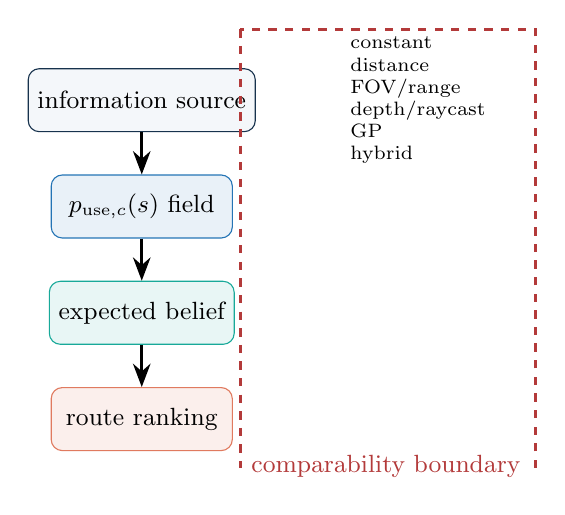
\begin{tikzpicture}[font=\small,>=Stealth]
        \node[draw=Navy,rounded corners,fill=Light,minimum width=2.3cm,minimum height=0.8cm] (src) at (0,3.0) {information source};
        \node[draw=Blue,rounded corners,fill=Blue!10,minimum width=2.3cm,minimum height=0.8cm] (field) at (0,1.65) {$\puse$ field};
        \node[draw=Teal,rounded corners,fill=Teal!10,minimum width=2.3cm,minimum height=0.8cm] (belief) at (0,0.3) {expected belief};
        \node[draw=Orange,rounded corners,fill=Orange!12,minimum width=2.3cm,minimum height=0.8cm] (route) at (0,-1.05) {route ranking};
        \draw[very thick,->] (src)--(field);
        \draw[very thick,->] (field)--(belief);
        \draw[very thick,->] (belief)--(route);
        \node[align=left,text width=2.1cm,font=\scriptsize] at (3.7,3.0) {constant\\distance\\FOV/range\\depth/raycast\\GP\\hybrid};
        \draw[Danger,dashed,very thick] (1.25,3.9) rectangle (5.0,-1.65);
        \node[Danger,fill=white] at (3.1,-1.65) {comparability boundary};
      \end{tikzpicture}
  \end{columns}
  \takeaway{A fair comparison changes the source of $p_{use}$, not the planner around it.}
\end{frame}

\begin{frame}{Shared pipeline: source $\rightarrow$ field $\rightarrow$ decision}
  \centering
  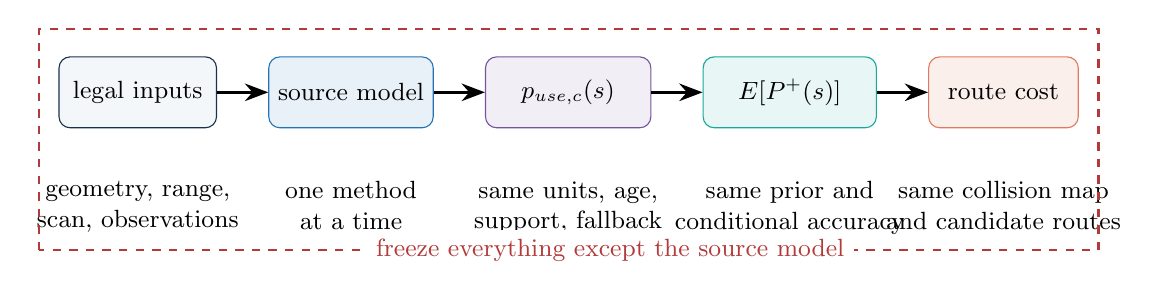
\begin{tikzpicture}[font=\small,>=Stealth,node distance=0.65cm]
    \node[draw=Navy,fill=Light,rounded corners,minimum width=2.0cm,minimum height=0.9cm] (input) {legal inputs};
    \node[draw=Blue,fill=Blue!10,rounded corners,minimum width=2.0cm,minimum height=0.9cm,right=of input] (source) {source model};
    \node[draw=Purple,fill=Purple!10,rounded corners,minimum width=2.1cm,minimum height=0.9cm,right=of source] (p) {$p_{use,c}(s)$};
    \node[draw=Teal,fill=Teal!10,rounded corners,minimum width=2.2cm,minimum height=0.9cm,right=of p] (post) {$E[P^+(s)]$};
    \node[draw=Orange,fill=Orange!12,rounded corners,minimum width=1.9cm,minimum height=0.9cm,right=of post] (plan) {route cost};
    \foreach \a/\b in {input/source,source/p,p/post,post/plan}{\draw[very thick,->] (\a)--(\b);}
    \node[below=0.55cm of input,align=center] {geometry, range,\\scan, observations};
    \node[below=0.55cm of source,align=center] {one method\\at a time};
    \node[below=0.55cm of p,align=center] {same units, age,\\support, fallback};
    \node[below=0.55cm of post,align=center] {same prior and\\conditional accuracy};
    \node[below=0.55cm of plan,align=center] {same collision map\\and candidate routes};
    \draw[Danger,dashed,thick] ($(input.south west)+(-.25,-1.55)$) rectangle ($(plan.north east)+(.25,.35)$);
    \node[Danger,fill=white] at (6.0,-2.0) {freeze everything except the source model};
  \end{tikzpicture}
  \vspace{0.45cm}
  \begin{block}{Two updates must stay separate}
    Runtime observations update the \textbf{robot belief}. Only learned/maintained sources update the
    \textbf{reliability field}. A detector hit is not automatically a map update.
  \end{block}
\end{frame}

\begin{frame}{Method 1 --- Conservative constant}
  \begin{columns}[T,onlytextwidth]
    \column{0.43\textwidth}
      \methodfacts{one prevalence $p_0$}{the same $p_{use}$ everywhere}{only at explicit recommissioning}{spatial structure matters}
      \[
        p_{use,c}(s)=p_0
      \]
    \column{0.54\textwidth}
      \centering
      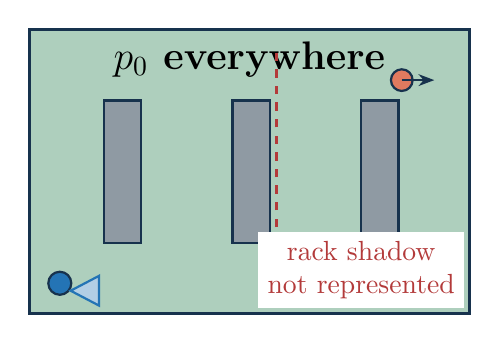
\begin{tikzpicture}[scale=0.86]
        \draw[fill=Green!45,draw=Navy,very thick] (0,0) rectangle (6.5,4.2);
        \foreach \x in {1.1,3.0,4.9}{\rack{\x}{1.05}}
        \camera{0.45}{0.45}\robot{5.5}{3.45}
        \node[font=\Large\bfseries] at (3.25,3.75) {$p_0$ everywhere};
        \draw[Danger,very thick,dashed] (3.65,0.3) -- (3.65,3.9);
        \node[Danger,align=center,fill=white] at (4.9,0.65) {rack shadow\\not represented};
      \end{tikzpicture}
  \end{columns}
  \takeaway{This is a necessary null model, not a straw man: complexity must beat it on held-out blocks.}
\end{frame}

\begin{frame}{Method 2 --- Distance-only}
  \begin{columns}[T,onlytextwidth]
    \column{0.43\textwidth}
      \methodfacts{camera position and a distance curve}{smooth radial reliability}{when the curve is recommissioned}{equal-range poses differ through orientation or occlusion}
      \[
        p_{use,c}(s)=f(\lVert s-c\rVert),\quad f'\le 0
      \]
    \column{0.54\textwidth}
      \centering
      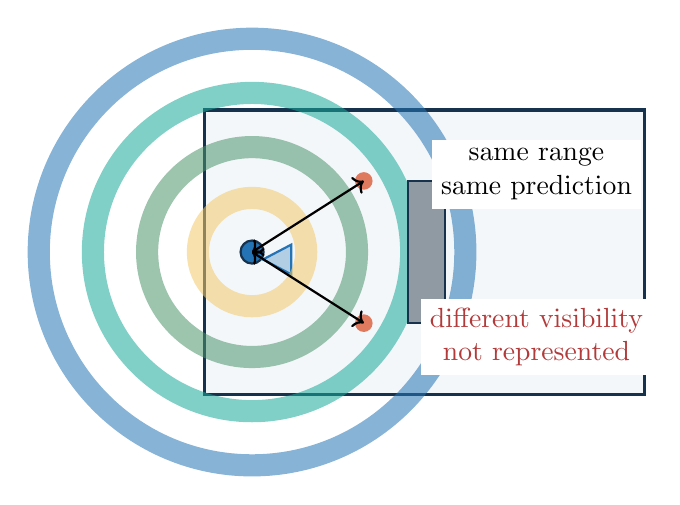
\begin{tikzpicture}[scale=0.86]
        \draw[fill=Light,draw=Navy,very thick] (0,0) rectangle (6.5,4.2);
        \camera{0.7}{2.1}
        \foreach \r/\c in {0.8/Yellow,1.55/Green,2.35/Teal,3.15/Blue}{\draw[\c,line width=8pt,opacity=.55] (0.7,2.1) circle (\r);}
        \rack{3.0}{1.05}
        \fill[Orange] (2.35,3.15) circle (.13);\fill[Orange] (2.35,1.05) circle (.13);
        \draw[<->,thick] (0.7,2.1)--(2.35,3.15);
        \draw[<->,thick] (0.7,2.1)--(2.35,1.05);
        \node[align=center,fill=white] at (4.9,3.25) {same range\\same prediction};
        \node[Danger,align=center,fill=white] at (4.9,.85) {different visibility\\not represented};
      \end{tikzpicture}
  \end{columns}
  \takeaway{Distance earns its place by revealing whether scene-aware inputs are actually necessary.}
\end{frame}

\begin{frame}{Method 3 --- Calibrated FOV and range}
  \begin{columns}[T,onlytextwidth]
    \column{0.43\textwidth}
      \methodfacts{camera pose, intrinsics, image bounds, target height}{analytic in-frustum/range score}{after calibration changes}{an obstacle blocks an otherwise valid ray}
      \[
        p_{use,c}(s)=g(\text{in-FOV},\text{range},\text{obliquity})
      \]
    \column{0.54\textwidth}
      \centering
      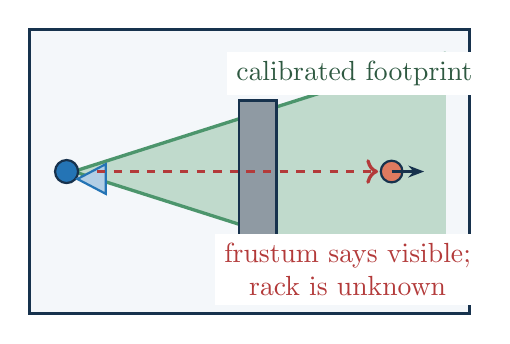
\begin{tikzpicture}[scale=0.86]
        \draw[fill=Light,draw=Navy,very thick] (0,0) rectangle (6.5,4.2);
        \fill[Green!35] (0.65,2.1) -- (6.15,.35) -- (6.15,3.85) -- cycle;
        \draw[Green,very thick] (0.65,2.1)--(6.15,.35) (0.65,2.1)--(6.15,3.85);
        \camera{0.55}{2.1}\rack{3.1}{1.05}\robot{5.35}{2.1}
        \draw[Danger,very thick,dashed,->] (1.0,2.1)--(5.15,2.1);
        \node[Danger,fill=white,align=center] at (4.7,.65) {frustum says visible;\\rack is unknown};
        \node[Green!60!black,fill=white] at (4.8,3.55) {calibrated footprint};
      \end{tikzpicture}
  \end{columns}
  \takeaway{FOV/range adds camera geometry, but not scene occlusion.}
\end{frame}

\begin{frame}{Method 4 --- Sensed depth and raycast}
  \begin{columns}[T,onlytextwidth]
    \column{0.43\textwidth}
      \methodfacts{camera calibration, sensed 3-D surface, target height, scan age}{line-of-sight reliability with unknown-cell fallback}{on rescan or declared live-depth update}{depth is missing, stale or misregistered}
      \small
      \[\text{depth}\rightarrow\text{point cloud}\rightarrow\text{height map}\rightarrow\text{raycast}\]
    \column{0.54\textwidth}
      \centering
      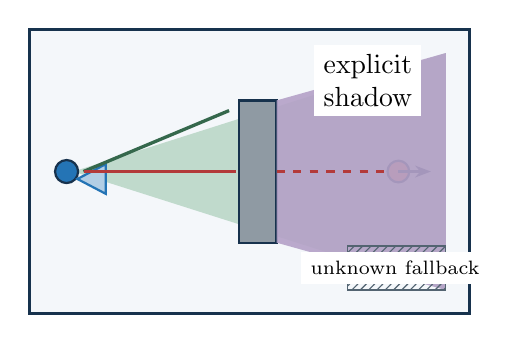
\begin{tikzpicture}[scale=0.86]
        \draw[fill=Light,draw=Navy,very thick] (0,0) rectangle (6.5,4.2);
        \fill[Green!35] (0.65,2.1) -- (6.15,.35) -- (6.15,3.85) -- cycle;
        \rack{3.1}{1.05}\camera{0.55}{2.1}\robot{5.45}{2.1}
        \fill[Purple!55,opacity=.9] (3.65,1.05) -- (6.15,.35) -- (6.15,3.85) -- (3.65,3.15) -- cycle;
        \draw[Green!70!black,very thick] (0.8,2.1)--(2.95,3.0);
        \draw[Danger,very thick] (0.8,2.1)--(3.05,2.1);
        \draw[Danger,very thick,dashed] (3.65,2.1)--(5.25,2.1);
        \node[fill=white,align=center] at (5.0,3.45) {explicit\\shadow};
        \draw[pattern=north east lines,pattern color=DarkGrey,draw=DarkGrey] (4.7,.35) rectangle (6.15,1.0);
        \node[font=\scriptsize,fill=white] at (5.4,.68) {unknown fallback};
      \end{tikzpicture}
  \end{columns}
  \takeaway{Depth provides cold-start occlusion structure, but it creates a freshness and missing-data obligation.}
\end{frame}

\begin{frame}{Method 5 --- Operational Gaussian process}
  \begin{columns}[T,onlytextwidth]
    \column{0.43\textwidth}
      \methodfacts{pose-labelled usable/miss blocks for each camera}{posterior mean plus separate epistemic support}{when eligible operational blocks arrive}{sharp boundaries or unsupported space are smoothed/extrapolated}
      \small
      \[f_c(s)\sim\mathcal{GP}(m_c,k_c),\qquad p_{use}=\sigma(f_c)\]
    \column{0.54\textwidth}
      \centering
      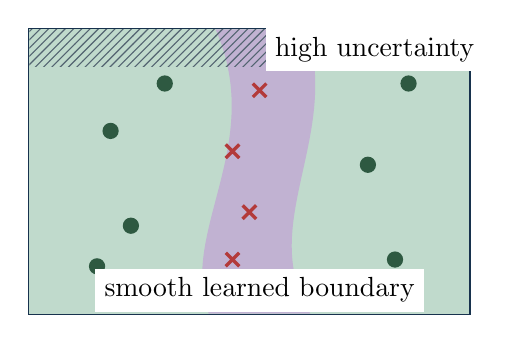
\begin{tikzpicture}[scale=0.86]
        \draw[fill=Light,draw=Navy,very thick] (0,0) rectangle (6.5,4.2);
        \fill[Green!35] (0,0) rectangle (6.5,4.2);
        \fill[Purple!45] (2.65,0) .. controls (2.2,1.2) and (3.5,2.5) .. (2.75,4.2) -- (4.1,4.2) .. controls (4.6,2.6) and (3.35,1.3) .. (4.15,0) -- cycle;
        \foreach \x/\y in {1.0/.7,1.5/1.3,1.2/2.7,2.0/3.4,5.4/.8,5.0/2.2,5.6/3.4}{\fill[Green!60!black] (\x,\y) circle (.12);}
        \foreach \x/\y in {3.0/.8,3.25/1.5,3.0/2.4,3.4/3.3}{\draw[Danger,very thick] (\x-.1,\y-.1)--(\x+.1,\y+.1) (\x-.1,\y+.1)--(\x+.1,\y-.1);}
        \draw[pattern=north east lines,pattern color=DarkGrey,draw=none] (0,3.65) rectangle (6.5,4.2);
        \node[fill=white] at (5.1,3.9) {high uncertainty};
        \node[fill=white,align=center] at (3.4,.35) {smooth learned boundary};
      \end{tikzpicture}
  \end{columns}
  \takeaway{The GP can learn installed-view effects, but repeated frames do not create new spatial support.}
\end{frame}

\begin{frame}{Method 6 --- Hybrid geometry plus learned residual}
  \begin{columns}[T,onlytextwidth]
    \column{0.43\textwidth}
      \methodfacts{depth/raycast prior plus operational blocks}{calibrated geometric prior corrected by a supported residual}{residual on observations; geometry on rescan}{a stale confident prior overwhelms sparse contradictory data}
      \small
      \[\operatorname{logit}p_{use}=\operatorname{logit}p_{depth}+r_{GP}\]
    \column{0.54\textwidth}
      \centering
      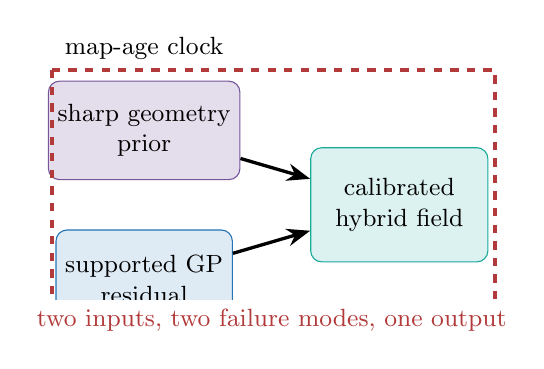
\begin{tikzpicture}[font=\small,>=Stealth,scale=0.9]
        \node[draw=Purple,fill=Purple!20,rounded corners,align=center,minimum width=2.0cm,minimum height=1.25cm] (geo) at (0,2.5) {sharp geometry\\prior};
        \node[draw=Blue,fill=Blue!15,rounded corners,align=center,minimum width=2.0cm,minimum height=1.25cm] (gp) at (0,.4) {supported GP\\residual};
        \node[draw=Teal,fill=Teal!15,rounded corners,align=center,minimum width=2.25cm,minimum height=1.45cm] (sum) at (3.6,1.45) {calibrated\\hybrid field};
        \draw[very thick,->] (geo)--(sum);\draw[very thick,->] (gp)--(sum);
        \node[above=.15cm of geo] {map-age clock};
        \draw[Danger,dashed,very thick] (-1.3,3.35) rectangle (4.95,-.18);
        \node[Danger,fill=white] at (1.8,-.18) {two inputs, two failure modes, one output};
      \end{tikzpicture}
  \end{columns}
  \takeaway{Freeze the candidate equation and reset rule first; hybrid must then beat both parents at equal budget.}
\end{frame}

\begin{frame}{Reference --- Complete CAD raycast}
  \begin{columns}[T,onlytextwidth]
    \column{0.43\textwidth}
      \methodfacts{complete simulator/SDF geometry and exact registration}{full static line-of-sight reference}{when oracle world truth changes}{its inputs are unavailable or stale in deployment}
      \vspace{0.3cm}
      \colorbox{Orange!25}{\parbox{.92\linewidth}{\centering\textbf{EVALUATION-ONLY ORACLE}\\Cannot win an operational comparison.}}
    \column{0.54\textwidth}
      \centering
      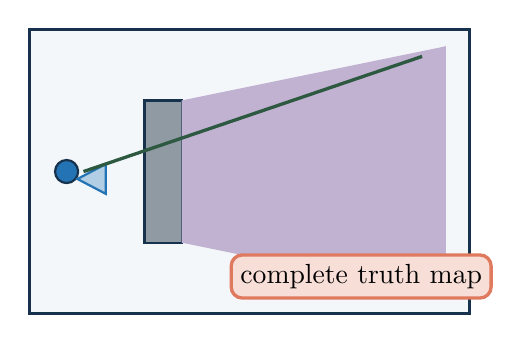
\begin{tikzpicture}[scale=0.86]
        \draw[fill=Light,draw=Navy,very thick] (0,0) rectangle (6.5,4.2);
        \camera{0.55}{2.1}
        \foreach \x in {1.7,3.1,4.5}{\rack{\x}{1.05}}
        \foreach \x/\y in {1.7/1.05,3.1/1.05,4.5/1.05}{
          \fill[Purple!45] (\x+.55,\y) -- (6.15,.25) -- (6.15,3.95) -- (\x+.55,\y+2.1) -- cycle;}
        \draw[Green!60!black,very thick] (.8,2.1)--(5.8,3.8);
        \node[fill=Orange!25,draw=Orange,very thick,rounded corners] at (4.9,.55) {complete truth map};
      \end{tikzpicture}
  \end{columns}
  \takeaway{CAD measures the geometric ceiling and diagnoses operational methods; it is not free deployment knowledge.}
\end{frame}

\begin{frame}{Source methods side by side}
  \scriptsize
  \renewcommand{\arraystretch}{1.22}
  \begin{tabular}{>{\raggedright\arraybackslash\bfseries}p{2.15cm}>{\raggedright\arraybackslash}p{3.45cm}>{\raggedright\arraybackslash}p{3.2cm}>{\raggedright\arraybackslash}p{4.1cm}}
    \toprule
    Method & Starts with & Changes when & Characteristic failure \\
    \midrule
    Constant & prevalence & recommissioned & no spatial structure \\
    Distance & camera position + curve & curve is refitted & ignores orientation and occlusion \\
    FOV/range & calibrated projection & camera is recalibrated & sees through obstacles \\
    Depth/raycast & sensed 3-D scan & geometry is rescanned & missing, stale or misregistered geometry \\
    Operational GP & prior + usable/miss blocks & new independent blocks arrive & smooth extrapolation in unsupported space \\
    Hybrid & depth prior + residual model & either input clock changes & stale prior conflicts with learned residual \\
    CAD reference & complete simulator truth & oracle world changes & non-operational input \\
    \bottomrule
  \end{tabular}
  \takeaway{The comparison is about information, maintenance and failure modes---not only predictive score.}
\end{frame}

\begin{frame}{Do not mix estimation with camera management}
  \centering
  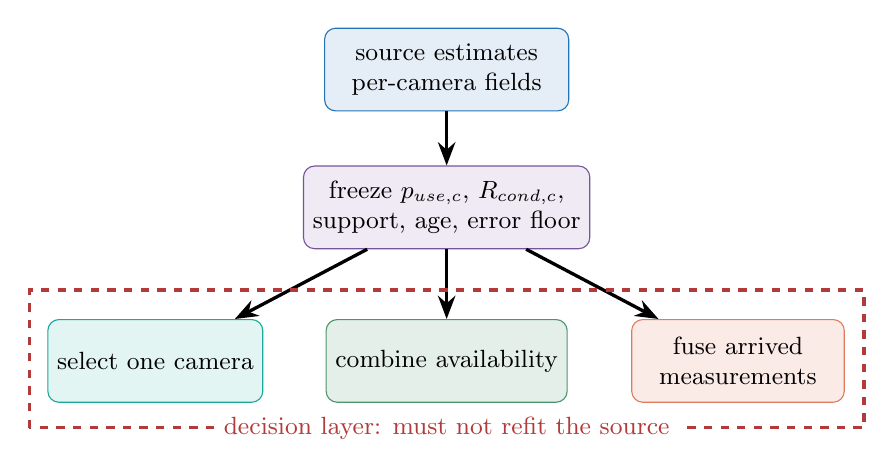
\begin{tikzpicture}[font=\small,>=Stealth]
    \node[draw=Blue,fill=Blue!12,rounded corners,align=center,minimum width=3.1cm,minimum height=1.05cm] (est) at (0,2.5) {source estimates\\per-camera fields};
    \node[draw=Purple,fill=Purple!12,rounded corners,align=center,minimum width=3.1cm,minimum height=1.05cm] (freeze) at (0,.75) {freeze $p_{use,c}$, $R_{cond,c}$,\\support, age, error floor};
    \node[draw=Teal,fill=Teal!12,rounded corners,minimum width=2.7cm,minimum height=1.05cm] (select) at (-3.7,-1.2) {select one camera};
    \node[draw=Green,fill=Green!15,rounded corners,minimum width=2.7cm,minimum height=1.05cm] (avail) at (0,-1.2) {combine availability};
    \node[draw=Orange,fill=Orange!15,rounded corners,align=center,minimum width=2.7cm,minimum height=1.05cm] (meas) at (3.7,-1.2) {fuse arrived\\measurements};
    \draw[very thick,->] (est)--(freeze);
    \draw[very thick,->] (freeze)--(select);
    \draw[very thick,->] (freeze)--(avail);
    \draw[very thick,->] (freeze)--(meas);
    \draw[Danger,dashed,very thick] (-5.3,-2.05) rectangle (5.3,-.3);
    \node[Danger,fill=white] at (0,-2.05) {decision layer: must not refit the source};
  \end{tikzpicture}
  \takeaway{A source can be good while a downstream selection/fusion policy is poor, and vice versa.}
\end{frame}

\begin{frame}{Decision method A --- Select one camera}
  \begin{columns}[T,onlytextwidth]
    \column{0.43\textwidth}
      \methodfacts{frozen per-camera fields}{one camera identity per candidate pose}{when health or candidate pose changes}{the chosen scalar ignores accuracy, correlation or switching cost}
      \begin{itemize}
        \item max availability: $\arg\max_c p_{use,c}$
        \item achievable precision: $\arg\min_c \sigma_{achievable,c}$
        \item hysteresis prevents rapid switching
      \end{itemize}
    \column{0.54\textwidth}
      \centering
      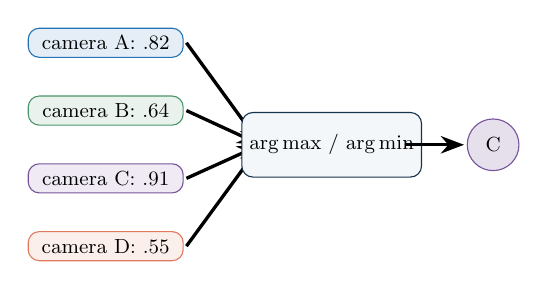
\begin{tikzpicture}[font=\small,>=Stealth,scale=.82,transform shape]
        \foreach \y/\name/\val/\col in {3.3/A/.82/Blue,2.25/B/.64/Green,1.2/C/.91/Purple,.15/D/.55/Orange}{
          \node[draw=\col,fill=\col!12,rounded corners,minimum width=2.4cm] (\name) at (0,\y) {camera \name: \val};
          \draw[very thick,->] (1.25,\y)--(2.4,1.72);}
        \node[draw=Navy,fill=Light,rounded corners,minimum width=2.2cm,minimum height=1cm] at (3.5,1.72) {$\arg\max$ / $\arg\min$};
        \draw[very thick,->] (4.65,1.72)--(5.55,1.72);
        \node[draw=Purple,fill=Purple!18,circle,minimum size=.8cm] at (6.0,1.72) {C};
      \end{tikzpicture}
  \end{columns}
  \takeaway{Selection is interpretable and correlation-safe, but discards simultaneous complementary measurements.}
\end{frame}

\begin{frame}{Decision method B --- Combine availability fields}
  \begin{columns}[T,onlytextwidth]
    \column{0.43\textwidth}
      \methodfacts{frozen per-camera usable-observation probabilities}{probability that at least one usable observation arrives}{when a component field/health changes}{camera events are treated as independent when they are correlated}
    \column{0.54\textwidth}
      \centering
      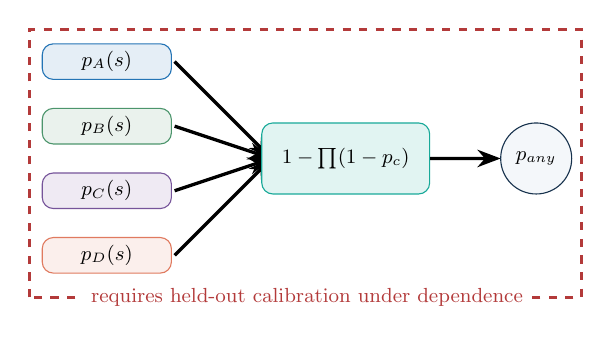
\begin{tikzpicture}[font=\small,>=Stealth,scale=.82,transform shape]
        \foreach \y/\name/\col in {3.2/A/Blue,2.2/B/Green,1.2/C/Purple,.2/D/Orange}{
          \node[draw=\col,fill=\col!12,rounded corners,minimum width=2cm] (\name) at (0,\y) {$p_{\name}(s)$};
          \draw[very thick,->] (1.05,\y)--(2.55,1.7);}
        \node[draw=Teal,fill=Teal!13,rounded corners,minimum width=2.6cm,minimum height=1.1cm] (or) at (3.7,1.7) {$1-\prod(1-p_c)$};
        \draw[very thick,->] (or)--(6.1,1.7);
        \node[draw=Navy,fill=Light,circle,minimum size=1.1cm] at (6.65,1.7) {$p_{any}$};
        \draw[Danger,dashed,very thick] (-1.2,-.45) rectangle (7.35,3.7);
        \node[Danger,fill=white] at (3.1,-.45) {requires held-out calibration under dependence};
      \end{tikzpicture}
  \end{columns}
  \takeaway{Noisy-OR is a probability rule, not measurement fusion; dependence must earn held-out calibration.}
\end{frame}

\begin{frame}{Decision method C --- Fuse arrived measurements}
  \begin{columns}[T,onlytextwidth]
    \column{0.43\textwidth}
      \methodfacts{actual time-aligned camera measurements and covariances}{one state correction}{at each realized measurement event}{shared systematic error is counted repeatedly}
      \begin{itemize}
        \item best-camera selection;
        \item naive independent sequential fusion;
        \item health-aware suppression / conservative floor.
      \end{itemize}
    \column{0.54\textwidth}
      \centering
      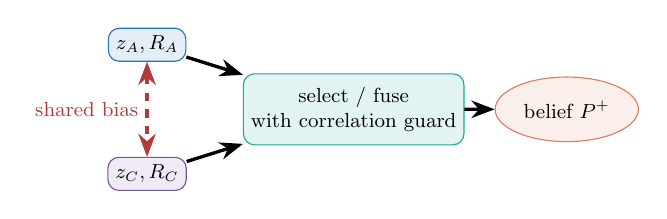
\begin{tikzpicture}[font=\small,>=Stealth,scale=.82,transform shape]
        \node[draw=Blue,fill=Blue!12,rounded corners] (za) at (0,2.7) {$z_A,R_A$};
        \node[draw=Purple,fill=Purple!12,rounded corners] (zc) at (0,.7) {$z_C,R_C$};
        \node[draw=Teal,fill=Teal!12,rounded corners,align=center,minimum width=2.6cm,minimum height=1.1cm] (f) at (3.2,1.7) {select / fuse\\with correlation guard};
        \node[draw=Orange,fill=Orange!12,ellipse,minimum width=2cm,minimum height=1cm] (b) at (6.5,1.7) {belief $P^+$};
        \draw[very thick,->] (za)--(f);\draw[very thick,->] (zc)--(f);\draw[very thick,->] (f)--(b);
        \draw[Danger,very thick,dashed,<->] (za)--node[left]{shared bias}(zc);
      \end{tikzpicture}
  \end{columns}
  \takeaway{More measurements do not guarantee more information when their errors share a cause.}
\end{frame}

\begin{frame}{Planner approximation 1 --- Precision blend}
  \begin{columns}[T,onlytextwidth]
    \column{0.43\textwidth}
      \methodfacts{$p_{use}$ plus visible/miss covariance endpoints}{one effective measurement covariance}{at every candidate state}{a miss is represented as a weak measurement instead of no measurement}
      \small
      \[
        R_{blend}^{-1}=pR_{hit}^{-1}+(1-p)R_{miss}^{-1}
      \]
    \column{0.54\textwidth}
      \centering
      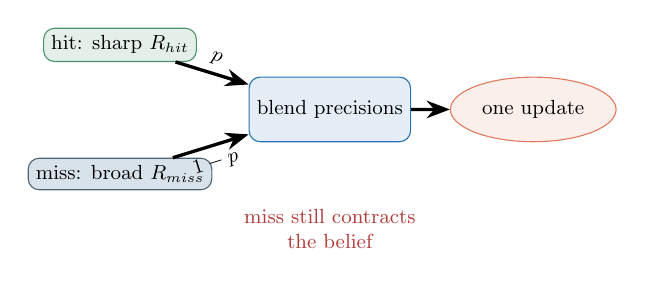
\begin{tikzpicture}[font=\small,>=Stealth,scale=.82,transform shape]
        \node[draw=Green,fill=Green!15,rounded corners] (hit) at (0,2.7) {hit: sharp $R_{hit}$};
        \node[draw=DarkGrey,fill=Mid,rounded corners] (miss) at (0,.7) {miss: broad $R_{miss}$};
        \node[draw=Blue,fill=Blue!12,rounded corners,minimum width=2.5cm,minimum height=1cm] (blend) at (3.25,1.7) {blend precisions};
        \node[draw=Orange,fill=Orange!12,ellipse,minimum width=2.1cm,minimum height=1cm] (update) at (6.4,1.7) {one update};
        \draw[very thick,->] (hit)--node[above,sloped]{$p$}(blend);
        \draw[very thick,->] (miss)--node[below,sloped]{$1-p$}(blend);
        \draw[very thick,->] (blend)--(update);
        \node[Danger,align=center,fill=white] at (3.25,-.15) {miss still contracts\\the belief};
      \end{tikzpicture}
  \end{columns}
  \takeaway{Computationally simple, but it collapses a discrete hit/miss event into one Gaussian promise.}
\end{frame}

\begin{frame}{Planner approximation 2 --- Scale covariance by $1/p$}
  \begin{columns}[T,onlytextwidth]
    \column{0.43\textwidth}
      \methodfacts{$p_{use}$ and conditional covariance $R$}{one inflated covariance $R/p$}{at every candidate state}{the equivalent covariance also depends on the prior belief}
      \[
        R_{eff}=R_{cond}/p_{use}
      \]
      \color{Danger}No pose-only cached $R_{eff}(s)$ can be exact for all priors.
    \column{0.54\textwidth}
      \centering
      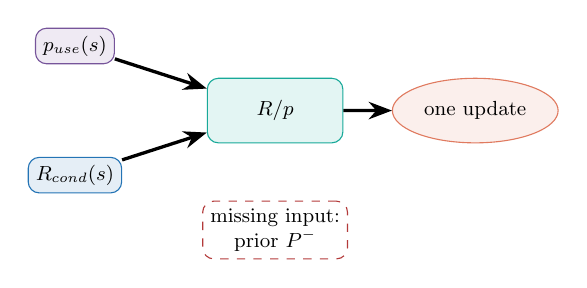
\begin{tikzpicture}[font=\small,>=Stealth,scale=.82,transform shape]
        \node[draw=Purple,fill=Purple!12,rounded corners] (p) at (0,2.7) {$p_{use}(s)$};
        \node[draw=Blue,fill=Blue!12,rounded corners] (r) at (0,.7) {$R_{cond}(s)$};
        \node[draw=Teal,fill=Teal!12,rounded corners,minimum width=2.1cm,minimum height=1cm] (div) at (3.1,1.7) {$R/p$};
        \node[draw=Orange,fill=Orange!12,ellipse,minimum width=2cm,minimum height=1cm] (u) at (6.2,1.7) {one update};
        \draw[very thick,->] (p)--(div);\draw[very thick,->] (r)--(div);\draw[very thick,->] (div)--(u);
        \node[draw=Danger,dashed,rounded corners,align=center] at (3.1,-.15) {missing input:\\prior $P^-$};
      \end{tikzpicture}
  \end{columns}
  \takeaway{$R/p$ is endpoint-correct but structurally cannot reproduce the expected branch for every prior.}
\end{frame}

\begin{frame}{Planner method 3 --- Explicit expected hit/miss branch}
  \begin{columns}[T,onlytextwidth]
    \column{0.43\textwidth}
      \methodfacts{$p_{use}$, $R_{cond}$ and prior $P^-$}{expected posterior covariance}{for every candidate state and current prior}{the source probabilities or conditional covariance are miscalibrated}
      \small\textbf{Rule:} $E[P^+]=p_{use}P_{hit}+(1-p_{use})P^-$.\\[0.15cm]
      A miss performs \textbf{no update}.
    \column{0.54\textwidth}
      \centering
      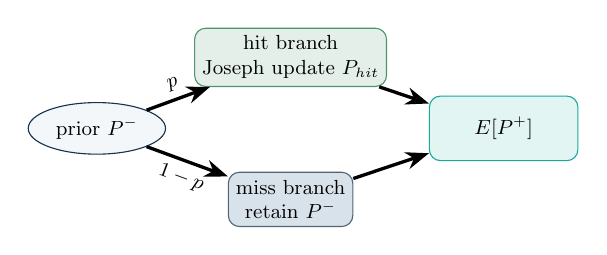
\begin{tikzpicture}[font=\small,>=Stealth,scale=.82,transform shape]
        \node[draw=Navy,fill=Light,ellipse] (prior) at (0,1.7) {prior $P^-$};
        \node[draw=Green,fill=Green!15,rounded corners,align=center] (hit) at (3.0,2.8) {hit branch\\Joseph update $P_{hit}$};
        \node[draw=DarkGrey,fill=Mid,rounded corners,align=center] (miss) at (3.0,.6) {miss branch\\retain $P^-$};
        \node[draw=Teal,fill=Teal!12,rounded corners,minimum width=2.3cm,minimum height=1cm] (e) at (6.3,1.7) {$E[P^+]$};
        \draw[very thick,->] (prior)--node[above,sloped]{$p$}(hit);
        \draw[very thick,->] (prior)--node[below,sloped]{$1-p$}(miss);
        \draw[very thick,->] (hit)--(e);\draw[very thick,->] (miss)--(e);
      \end{tikzpicture}
  \end{columns}
  \takeaway{This preserves the event semantics: usable observation or no observation.}
\end{frame}

\begin{frame}{Belief containment --- Persistent-error correlation floor}
  \begin{columns}[T,onlytextwidth]
    \column{0.43\textwidth}
      \methodfacts{fresh held-out residual blocks grouped by camera/site}{a lower bound on measurement uncertainty plus cross-camera check}{only after fresh commissioning and lifecycle validation}{the floor is learned from confounded or stale residuals}
      \[
        R_{used,c}(s)\succeq R_{floor,c}
      \]
      This is containment, not proof that the bias source is camera calibration.
    \column{0.54\textwidth}
      \centering
      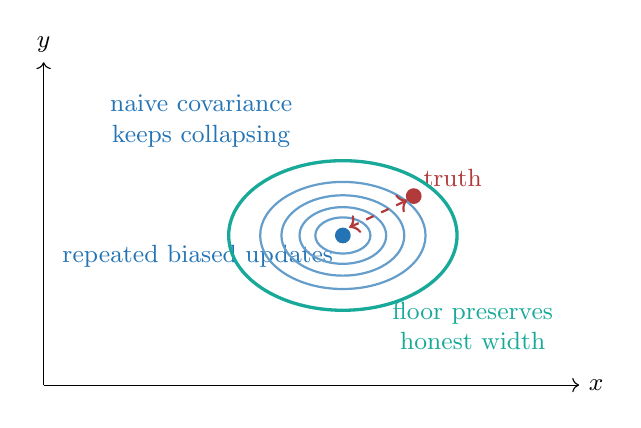
\begin{tikzpicture}[font=\small]
        \draw[->] (0,0)--(6.8,0) node[right]{$x$};
        \draw[->] (0,0)--(0,4.1) node[above]{$y$};
        \fill[Danger] (4.7,2.4) circle (.1) node[above right]{truth};
        \fill[Blue] (3.8,1.9) circle (.1) node[below left]{repeated biased updates};
        \foreach \r/\ry in {1.05/.68,.78/.51,.55/.36,.35/.23}{\draw[Blue!70,thick] (3.8,1.9) ellipse (\r cm and \ry cm);}
        \draw[Teal,very thick] (3.8,1.9) ellipse (1.45 and .95);
        \draw[Danger,dashed,thick,<->] (3.88,2.0)--(4.62,2.35);
        \node[Blue,align=center] at (2.0,3.35) {naive covariance\\keeps collapsing};
        \node[Teal,align=center] at (5.45,.75) {floor preserves\\honest width};
      \end{tikzpicture}
  \end{columns}
  \takeaway{The floor prevents false confidence; fresh identifiability is still required before attributing its source.}
\end{frame}

\begin{frame}{What is fresh, and what is not evidence yet?}
  \begin{columns}[T,onlytextwidth]
    \column{0.48\textwidth}
      \begin{block}{This deck}
        \begin{itemize}
          \item New vector schematics only
          \item No old captures, runs, fits or plots
          \item Explains mechanisms and decision boundaries
          \item Makes no ranking or navigation claim
        \end{itemize}
      \end{block}
    \column{0.48\textwidth}
      \begin{block}{Fresh evidence still required}
        \begin{itemize}
          \item 6 sites $\times$ 8 yaws $\times$ 2 sessions
          \item 96 capture blocks; A--D simultaneous
          \item site-grouped analysis, never frame inference
          \item fresh source benchmark on shared blocks
          \item complete manifests and hashes
        \end{itemize}
      \end{block}
  \end{columns}
  \vspace{0.35cm}
  \centering
  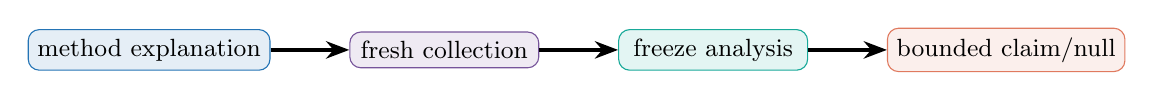
\begin{tikzpicture}[font=\small,>=Stealth]
    \node[draw=Blue,fill=Blue!12,rounded corners,minimum width=2.4cm] (explain) {method explanation};
    \node[draw=Purple,fill=Purple!12,rounded corners,minimum width=2.4cm,right=1.0cm of explain] (collect) {fresh collection};
    \node[draw=Teal,fill=Teal!12,rounded corners,minimum width=2.4cm,right=1.0cm of collect] (freeze) {freeze analysis};
    \node[draw=Orange,fill=Orange!12,rounded corners,minimum width=2.4cm,right=1.0cm of freeze] (claim) {bounded claim/null};
    \foreach \a/\b in {explain/collect,collect/freeze,freeze/claim}{\draw[very thick,->] (\a)--(\b);}
  \end{tikzpicture}
\end{frame}

\begin{frame}{Decisions requested from the supervisor}
  \begin{enumerate}\setlength\itemsep{0.65em}
    \item Is $p_{use,c}(s)$ the right common estimand and label definition?
    \item Which depth provenance is the primary operational arm: commissioning scan,
      live sensed depth, or commissioned static map?
    \item Is the hybrid candidate form acceptable, and what reset/decay rule follows a rescan?
    \item Approve or amend the fresh 6-site $\times$ 8-yaw $\times$ 2-session identifiability design
      and its practical-effect/harm gates.
    \item Which single endpoint should govern a later matched closed-loop campaign, if the
      identifiability gate passes?
  \end{enumerate}
  \vspace{0.25cm}
  \begin{beamercolorbox}[wd=\linewidth,sep=.2cm,rounded=true]{block body}
    \centering\large\textbf{Proposed meeting outcome: freeze the comparison contract, not a winner.}
  \end{beamercolorbox}
\end{frame}

\end{document}
